\documentclass[acmtog]{acmart}
\usepackage{graphicx}
\usepackage{subfigure}
\usepackage{natbib}
\usepackage{listings}
\usepackage{bm}
\usepackage{amsmath}
\usepackage{graphicx}
% \usepackage[outercaption]{sidecap}
\graphicspath{ {./} }
\definecolor{blve}{rgb}{0.3372549 , 0.61176471, 0.83921569}
\definecolor{gr33n}{rgb}{0.29019608, 0.7372549, 0.64705882}
\makeatletter
\lst@InstallKeywords k{class}{classstyle}\slshape{classstyle}{}ld
\makeatother
\lstset{language=C++,
	basicstyle=\ttfamily,
	keywordstyle=\color{blve}\ttfamily,
	stringstyle=\color{red}\ttfamily,
	commentstyle=\color{magenta}\ttfamily,
	morecomment=[l][\color{magenta}]{\#},
	classstyle = \bfseries\color{gr33n}, 
	tabsize=2
}
\lstset{basicstyle=\ttfamily}

% Title portion
\title{Assignment 1:\\ Exploring OpenGL and Phong Lighting} 

\author{Name:\quad Bingnan Li  \\ student number:\ 2020533092
\\email:\quad libn@shanghaitech.edu.cn}

% Document starts
\begin{document}
\maketitle

\vspace*{2 ex}

\section{Introduction}
\begin{itemize}
\item Loading mesh file from .obj files has been done.
\item Customized camera systems based on Euler angles has been done.
\item Phong lighting system with ambient, diffuse and specular lights has been done.
\item Multi-lights and spotlights system has been done.
\item Play with geometry shader. 
\end{itemize}
\section{Implementation Details}
\begin{enumerate}	
	\setlength{\parindent}{2em}
	\item Loading mesh from .obj files:
	\par First loaded vertices into self.Vertices, then I loaded normal vectors into a temporary variable. Lastly, I merge them by the indices given by faces.
	\item VAO, VBO, EBO and shaders:
	\par I created VAO, VBO, EBO in mesh class, then I binded and transferred data to VBO and EBO.\par
	For shaders, I compiled shaders in shader class and link them to shader program.
	\item Camera system:\par
	I initialized yaw angle to -90 degree since we initially face to negative z direction. Then I use pitch and yaw angles to calculate Front variable, which is used to indicate the view direction. Then we set positive y direction unit vector as WorldUp variable to indicate the unchanged up direction in world coordinate. With Front and WorldUp, we can calculate Right base with cross product of Front and WorldUp. After that, we can get Up base by calculating cross product of Right and Front. Thus, we built the camera coordinates with (Front, Right, Up).\par
	Then I build the calling functions of keyboard inputs and Cursor movements. For forward and backward, leftward and rightward movements, upward and downward movements, camera position changes along Front, Right and Up vectors respectively. Then for cursor movements, I stored last cursor position in last frame and calculate difference with new cursor position. What needs to be specified is that the position that function "glfwSetCursorPosCallback" returns is the relative position from the left-up corner of display. Then we use the offset along two axes to adjust the value of Yaw and Pitch so that we can calculate new Front with those two angles.
	\item Phong lighting:\par
	Phong lighting has three components: ambient, diffuse and specular.\par For ambient light, I set an ambient strength to control the intensity of ambient light, then I multiply ambient strength with light color as the ambient light.\par
	For diffuse light, I calculated the dot product of inverse light direction and normal vector as the diffuse intensity, then I multiply this intensity with light color as diffuse light.\par
	For specular light, I first calculate the reflection light, then I calculated the dot product of reflection light and view direction. After that I calculated the 32 pow of this dot product in order to get a more smooth high light. Finally, I use multiply it with specular intensity and light color as specular light.\par
	Lastly, I added those three parts together and then multiply it with object color as the result color.
	\item Multi-light and spotlight system:\par
	I instantiated a new shader to render spheres in each light sources to represent real bodies of light sources.\par
	I render three kinds of lights: directional light, point light and spotlight moving with camera. For each kind of light, I build different render functions in fragment shader source file.\par
	First, for directional light, the corresponding rendering function is similar to basic phong lighting system.\par
	Second, for point light, I added a decay into the result light with distance. I firstly calculated the distance between fragment point and light source, then I applied \[attenuation = \frac{1}{K_0 + K_1 \times distance + K_2 * distance^2}\] to get the decay factor, then I multiply it with result to implement light intensity decay.\par
	Third, for spotlight, I firstly set light position to camera position and set light direction to camera Front so that the spotlight we move with camera. Then I set a cut-off angel to specify the range of lighting. For each fragment points, I determine whether it is in the range of the spotlight. In order to smooth light circle edge, I added an outer cut-off angle variable, for fragment position between cut-off angle and outer cut-off angle, the intensity of light we decay linearly.
	\item Play with geometry:\par   
	For each input triangle primes, I first calculated the geometry center of the prime by averaging three vertices, then I calculated a new normal vector by averaging three normal vectors of vertices. Next I translate the geometry center along with the outer normal direction. Then I add three new faces by combine any two of the three vertices and the new generated point. Finally, I calculated the corresponding normal vectors by cross product.
	
\end{enumerate}	
\section{Results}
\begin{figure}[h]
    \centering
    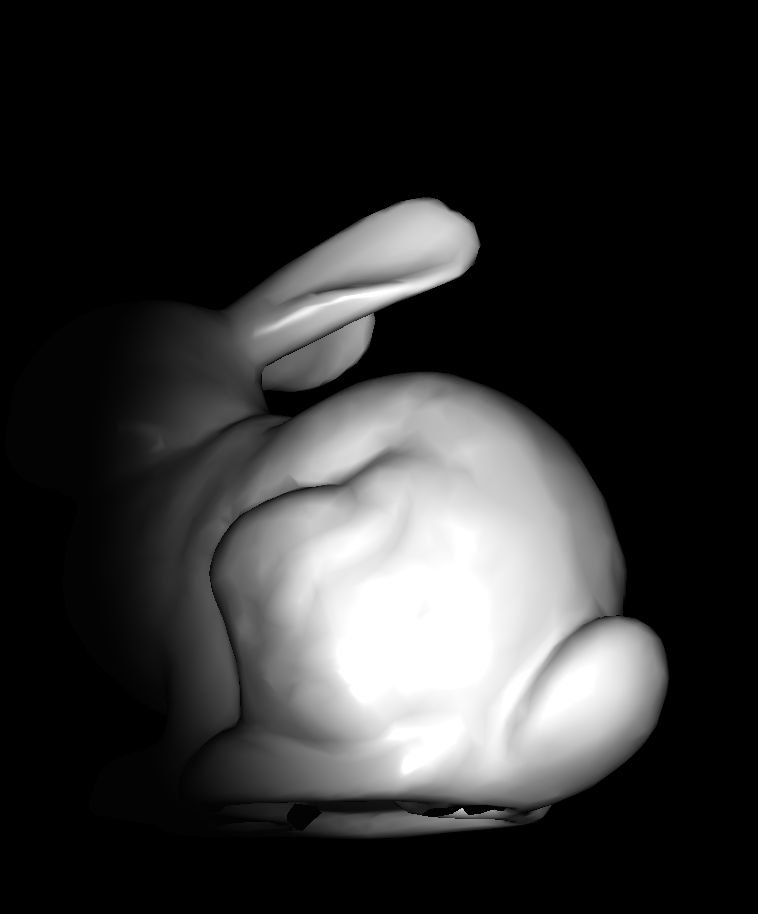
\includegraphics[width=0.4\textwidth]{bunny_with_spotlight_only}
    \caption{Bunny with only spotlight system and phong lighting system}
\end{figure}
% 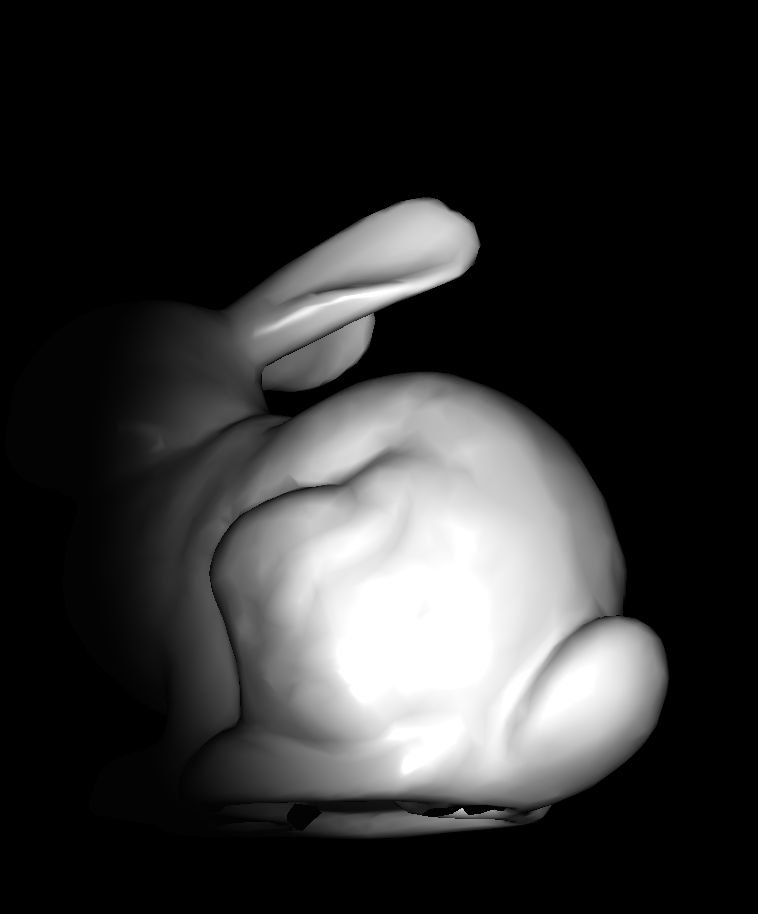
\includegraphics[scale=0.2]{bunny_with_spotlight_only}


\begin{figure}[h]
    \centering
    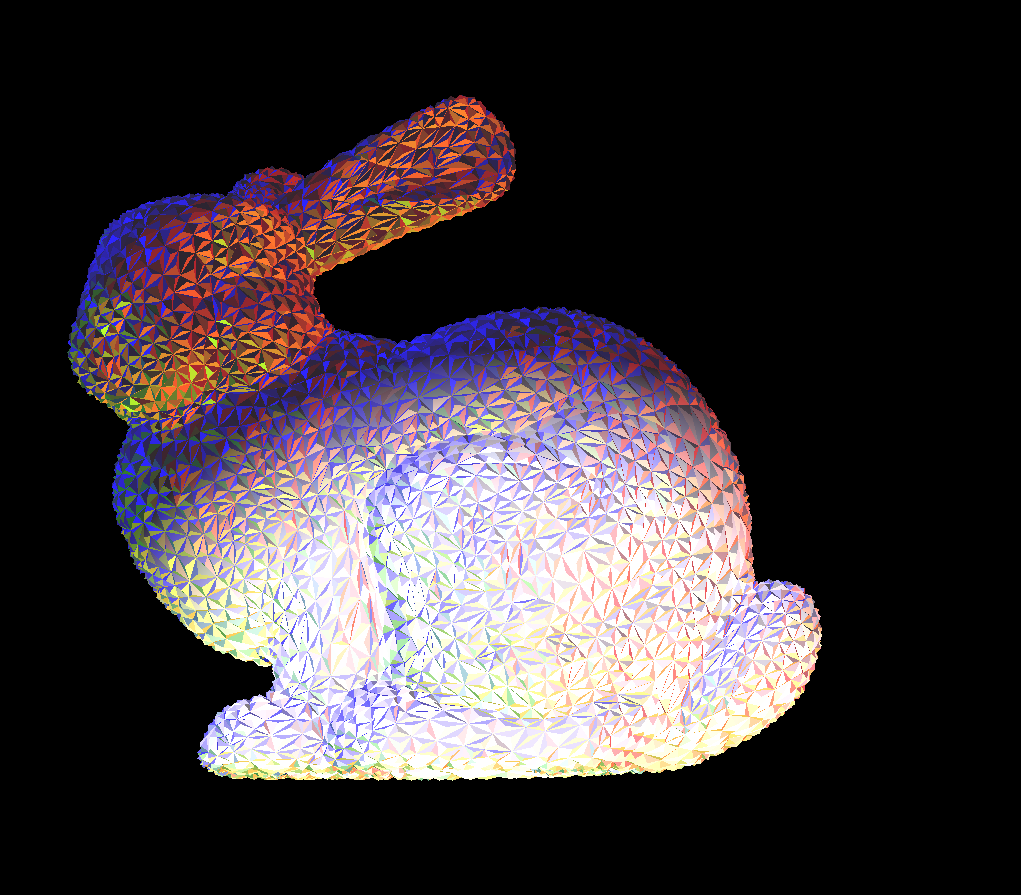
\includegraphics[width=0.4\textwidth]{bunny_with_geometry_multi_spot}
    \caption{Bunny with geometry shader and multi-light system}
\end{figure}

\begin{figure}[h]
    \centering
    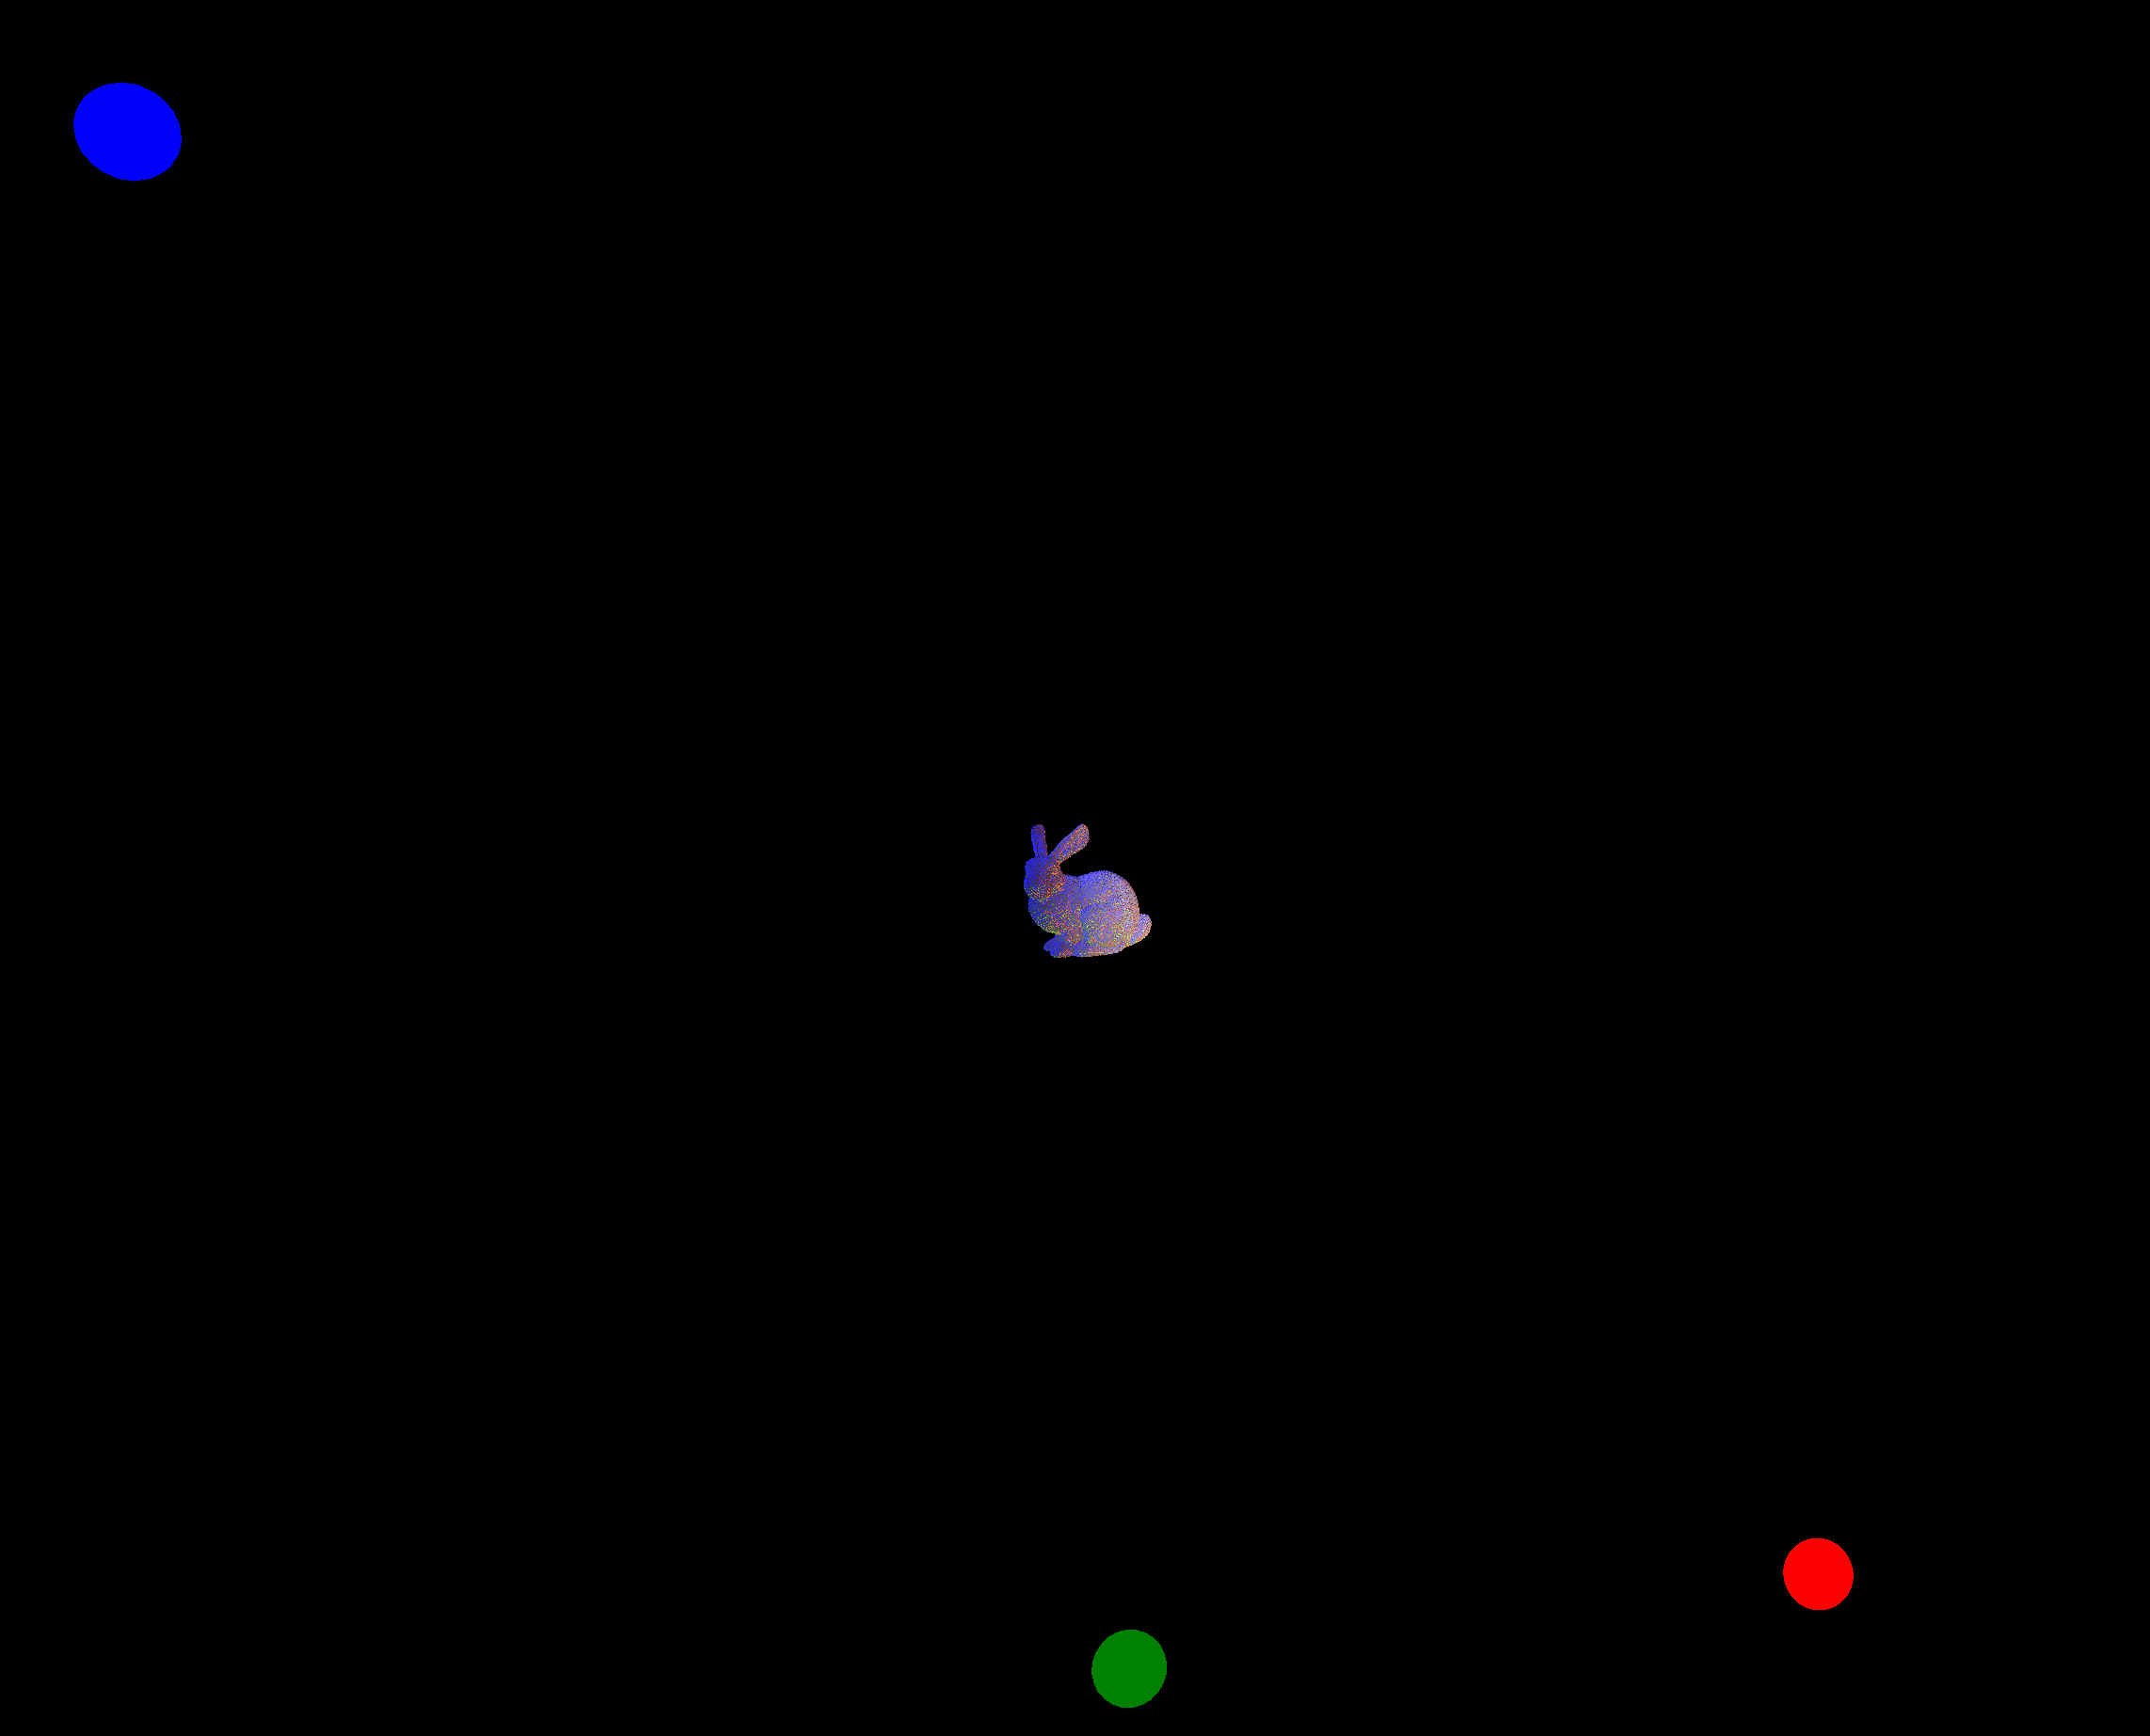
\includegraphics[width=0.4\textwidth]{overview}
    \caption{overview of the whole scene}
\end{figure}

\end{document}
